\section{Related Work}
\label{sec:related-work}

\subsection{TransFuser (2021)}
\label{sec:related-work:transfuser}
TransFuser, ranked 2nd when published and currently ranked 4th on the CARLA Leaderboard,
is an end-to-end approach to autonomous driving in the CARLA simulator
\cite{transfuser-pami, transfuser-cvpr, pwc-carla}.
In their paper, \textcite{transfuser-pami} explores how complementary sensors should be integrated for autonomous driving. Their model uses both RGB images and LIDAR data, and outputs position waypoints that are passed to a traditional PID-controller for steering.
By interleaving Transformer-blocks within both the RGB and LIDAR feature extraction branches,
features are fused between the two sensor modalities leading to exchange of information and supposed improved understanding of the environment. An overview of the architecture is shown in \cref{fig:transfuser-architecture}.

\begin{figure}[htbp]
    \centering
    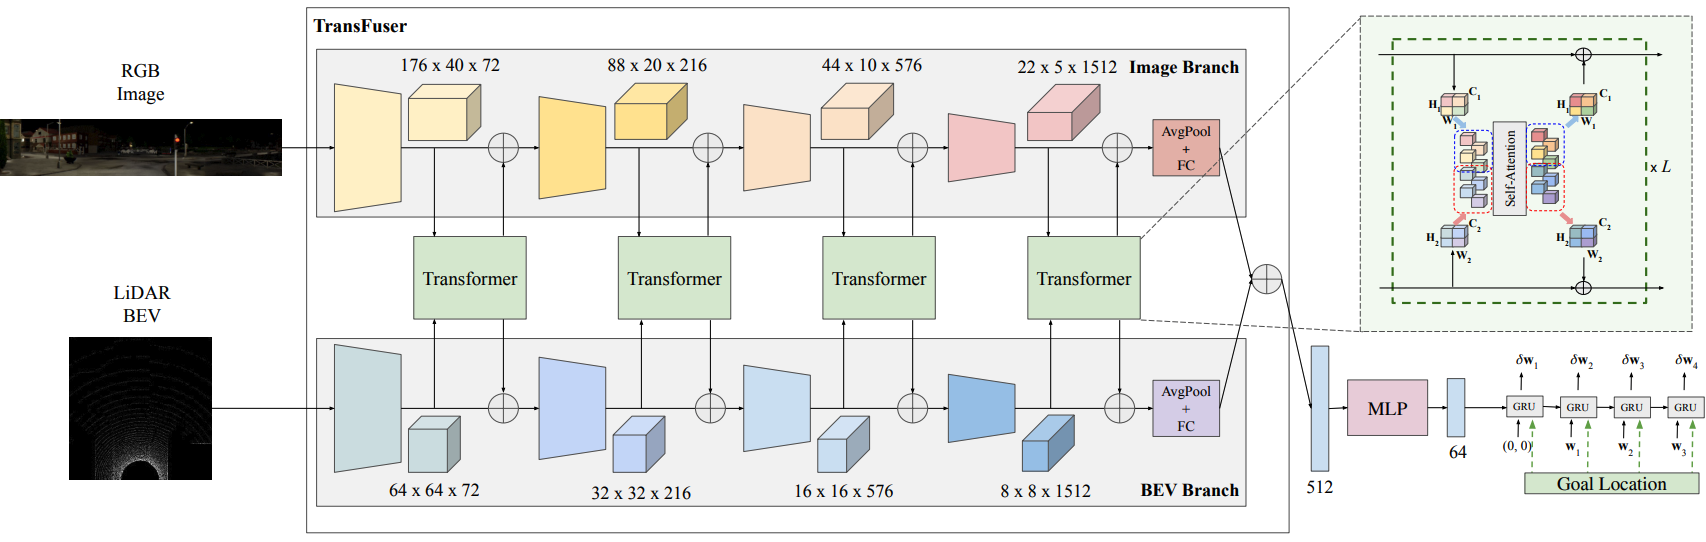
\includegraphics[width=\textwidth]{chapters/2-background/figures/transfuser-architecture.png}
    \caption{The TransFuser architecture uses several transformer modules for the fusion of intermediate feature maps between RGB and LIDAR data. The two branches are combined and fed into an MLP before passing it to an auto-regressive waypoint prediction network.  Source: \cite{transfuser-pami}.}
    \label{fig:transfuser-architecture}
\end{figure}

During training, TransFuser optimizes a multi-task loss consisting of not only predicting waypoints,
but also predicting depth and semantic segmentation images,
as well as a top-down HD-map and bounding boxes vehicle detection.

\textcite{transfuser-pami} also propose a new benchmark for autonomous driving called Longest6. This involves longer routes, increased traffic density and more challenging pre-crash scenarios than existing closed-loop driving benchmarks. Another advantage of this benchmark over the official CARLA Leaderboard is that it can be used for evaluation on local resources without the online platform's computation budget restrictions.

As this specialization project is based on TransFuser, a more detailed description of the model and benchmark can be found in \cref{sec:transfuser} and \cref{sec:evaluation} respectively.


\subsection{Learning from All Vehicles (2022)}
\textcite{chen2022lav} presents in their paper a system to train models for autonomous driving on data not just from the ego-vehicle itself, but also other vehicles it observes.
They argue that training on other vehicle's trajectories will help with sample efficiency, greatly increase the chance that the model sees interesting scenarios and help the ego-vehicle avoid collisions. Finding these trajectories are however challenging due to partial observability and the lack of sensors in other vehicles.

\begin{figure}[htbp]
    \centering
    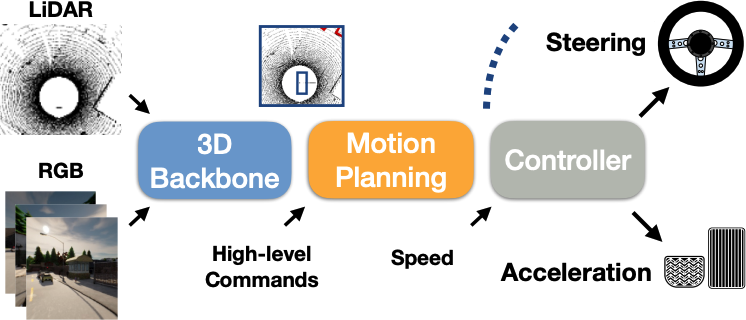
\includegraphics[width=.7\textwidth]{chapters/2-background/figures/lav.png}
    \caption{An overview of the Learning from All Vehicles inference architecture. It consists of three modules: A perception module, a motion planner and a low-level controller. Source: \cite{chen2022lav}.}
    \label{fig:lav}
\end{figure}

Their end-to-end model consists of a three-stage modular pipeline, as seen in \cref{fig:lav}. The first stage is a perception module that maps raw sensor readings from three front-facing RGB cameras and LIDAR to map-view feature representations. Its goal is to create a robust and generalizable representation of the surrounding world, and to build vehicle-invariant features that help supervise the motion planner. The motion planner is the second stage and it uses these features to produce a series of waypoints describing the future trajectory of all vehicles that surrounds the ego-vehicle. The last stage is a low-level controller that converts motion plans into actions to be executed on the vehicle. \textcite{chen2022lav} reached the top of the CARLA Leaderboard with their submitted paper, and is currently ranked 3rd \cite{chen2022lav, pwc-carla}.


\subsection{Trajectory-guided Control Prediction (TCP) (2022)}
blabla\todo introduces the idea of simultaneously predicting a desired trajectory and desired control outputs.
The


\subsection{InterFuser (2022)}
\textcite{shao2022interfuser} propose InterFuser, a safety-enhanced autonomous driving framework. They investigate methods for multi-modal sensor fusion in a more scalable and effective way than TransFuser's multi-stage approach. They also work towards interpretability of their end-to-end model by creating a safety mind map based on immediate features, which they argue can help unveil the model's decision basis and failure causes.

\begin{figure}[htbp]
    \centering
    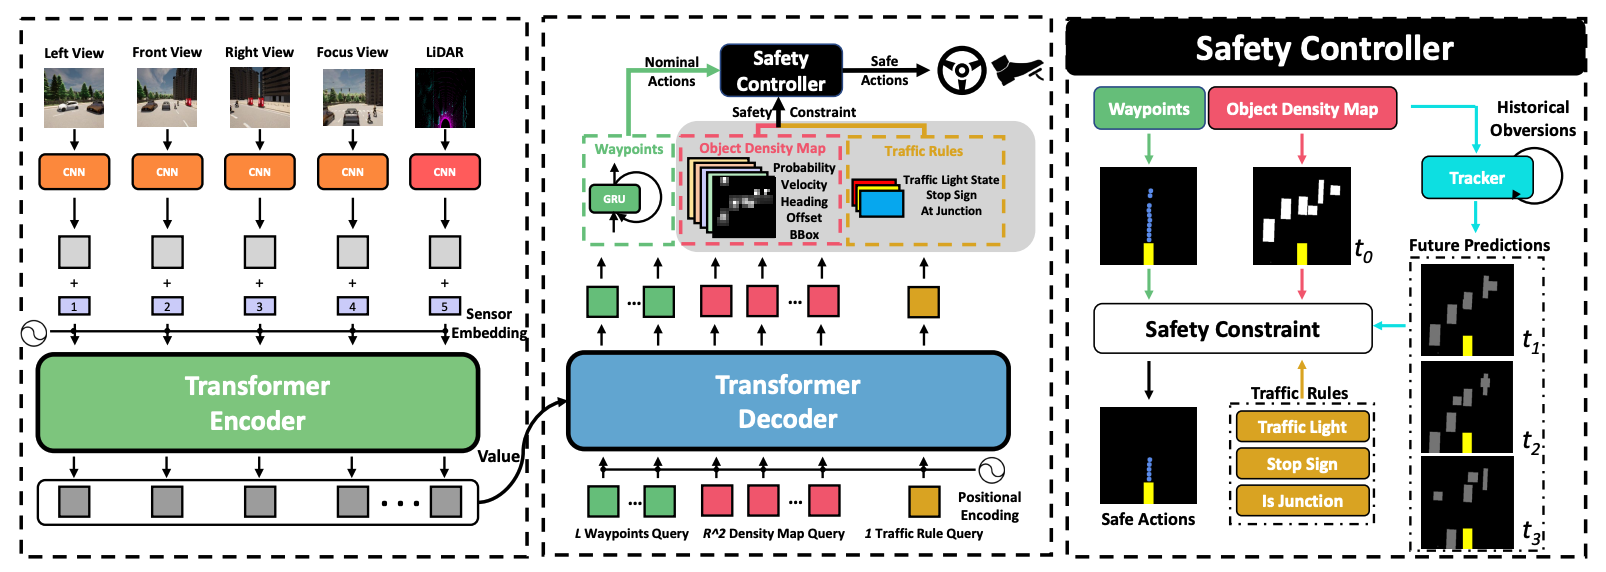
\includegraphics[width=\textwidth]{chapters/2-background/figures/interfuser.png}
    \caption{The InterFuser architecture. It consists of an encoder-decoder network built on transformers, in addition to a safety controller that constraints the output actions to enhance driving safety. Source: \cite{shao2022interfuser}.}
    \label{fig:interfuser}
\end{figure}

The models follows an encoder-decoder architecture as seen in \cref{fig:interfuser}. The input consists of three RGB cameras (left, front and right) and LIDAR. From the RGB cameras they create four images, one for each direction and one focusing-view image to capture distant traffic lights. The inputs are then fused in a multi-view multi-modal transformer before being fed into the decoder. The decoder takes queries in the form of waypoints, density maps and a traffic rule to the attention mechanism and outputs predictions of the same attributes. Finally, a safety controller uses the predicted waypoints, object density map and traffic rule to create a safety mind map, which is utilized to constrain the actions into a safe set. InterFuser is currently the top performer on the CARLA Leaderboard \cite{shao2022interfuser, pwc-carla}.
